\chapter{AdaptaMaterialEscolar 2.0}
\label{cap:AdaptaMaterialEscolar2.0}
En este capítulo explicaremos la obtención de requisitos y cómo se han clasificado en la Sección \ref{cap:requisitos}. También se describirá el diseño realizado por cada integrante de la aplicación para la iteración competitiva y el diseño final de las funcionalidades en la Sección \ref{disenyoDeLaAplicacion}.


\section{Requisitos}
\label{cap:requisitos}

Lo primero que hicimos fue analizar la memoria de AdaptaMaterialEscolar 1.0 (\cite*{AdaptaMaterialEscolar1.0}) extrayendo las funcionalidades que faltaban por implementar y los resultados de la evaluación que se realizó. Tras este análisis surgieron una serie de cambios y nuevas funcionalidades. Uno de los cambios fue agrupar dichas funcionalidades en formato (funcionalidades que tienen relación con el estilo o la estructura del documento), en ejercicios (funcionalidades relacionadas con la creación de actividades) y finalmente en auxiliar (resto de funcionalidades que no pertenecen a formato o a ejercicios). Quedan así las funcionalidades agrupadas de la siguiente manera:
\\

Funcionalidades relacionadas con el formato: 
\begin{itemize}
  \item Añadir encabezado al texto: El usuario eligirá un encabezado que se añadirá al docuemnto.
  \item Añadir un tipo de fuente escolar: Incluir en los tipos de fuentes la escolar. Dicha fuente se refleja en la Figura \ref{escolar}.
  \begin{figure}[ht!]
    \centering
    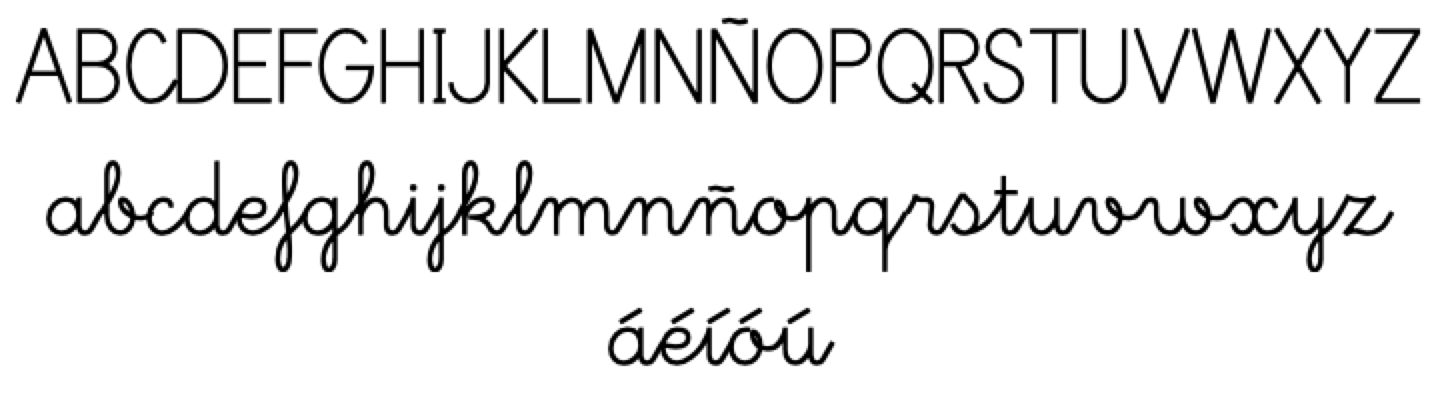
\includegraphics[scale=0.3]{AdaptaMaterialEscolar/FunteEscolar.png}
    \caption{Fuente escolar.}
    \label{escolar}
\end{figure}
  \item Añadir una leyenda de colores con la categoría de cada tipo: Crear una lista de conceptos asociados a un color.
  \item Añadir leyenda de colores para el tema de cada asignatura: Dar la posibilidad de que cada asignatura tenga un color. Al crear un documento según la asignatura se pondrá el borde del documento del color que corresponde a dicha asignatura.
  \item Añadir cuadrícula: En vez de renglones de una única línea se podrá poner para responder a una pregunta la cuadrícula.
  \item Añadir la opción de añadir doble pauta: En vez de renglones de una única línea se podrá poner para responder a una pregunta la doble pauta.
  \item Estandarizar formato para títulos e índices del temario: Dar la opción de crear estilos para estandarizar documento.
  \item Enumerar ejercicios de forma automática: Establecer un orden numérico para los ejercicios de forma automática según se van creando para que el usuario no se tenga que preocupar de ese aspecto.
\end{itemize}
Funcionalidades asociadas con la creación de ejercicios:
\begin{itemize}
  \item Ejercicios de relacionar contenido mediante flechas: Generar un ejercicio para relacionar conceptos mediante flechas.
  \item Añadir ejercicios de cálculo con huecos a rellenar por el alumno: Posibilidad de introducir ejercicios de cálculo con espacios en blanco para que el alumno rellene dichos huecos con contenido adecuado.
  \item Añadir ejercicios con espacio para dibujar: Añadir amplio hueco en blanco con el fin de que el alumno pueda dibujar.
  \item Ejercicios de completar los espacios en blanco en tablas y esquemas: Dada una tabla o un esquema se establecen espacios en blanco para que el alumno los rellene con el contenido adecuado.
\end{itemize}
Funcionalidades auxiliares:
\begin{itemize}
  \item Generar un resumen a partir de un texto.
  \item Exportar el documento a formato Word.
  \item Añadir un pictotraductor: Dada una frase traducirla a pictogramas.
  \item Añadir imágenes buscando una palabra: A partir de una palabra se busca su respectiva imagen en las bases de datos de imágenes libres.
  \item Sustituir una palabra por una imagen: Una palabra se reemplazará por una imagen.
  \item Crear una herramienta de recorte de imágenes: Tras seleccionar una imagen se dará la opción de quitar partes de la misma. 
  \item Crear tablas que organicen el temario y/o las actividades, seleccionando contenido: Tras la selección de contenido por parte del usuario se creará una tabla en base a la información seleccionada, con un formato predefinido.
  \item Creación de esquemas.
\end{itemize}
Tras haber analizado en detalle las funcionalidades anteriores hemos encontrado que varias funciones ya están implementadas en la versión original de AdaptaMaterialEscolar y otras hemos decidido no implementarlas ya que consideramos que no tenemos la información suficiente para ello. Las siguientes funcionalidades son las que ya están implementadas en la versión original:
  \begin{itemize}
    \item Añadir encabezado al texto: El documento editable tiene una opción con una lista de encabezados para añadir uno y cuando se pulsa un encabezado el documento editable convierte el formato de la letra en el del encabezado seleccionado. 
    \item Enumerar ejercicios de forma automática: El documento editable permite añadir listas enumeradas.
  \end{itemize}
Las funcionalidades que hemos decidido descartar de momento por falta de información son las siguientes:
\begin{itemize}
  \item Añadir imágenes buscando una palabra. Partimos de que debemos usar una base de datos de imagen libre pero no tenemos la información suficiente para definir cuál sería la base de datos correcta.
  \item Sustituir una palabra por una imagen.
  \item Crear una herramienta de recorte de imágenes para el texto original: No la realizaremos ya que no tenemos claro que tipo de recorte tenía pensado el usuario. 
  \item Crear tablas que organicen el temario y/o las actividades, seleccionando contenido: Descartamos dicha funcionalidad ya que no tenemos la información suficiente del formato que desea el usuario.
  \item Crear esquemas: Descartamos dicha funcionalidad ya que no tenemos la información suficiente del formato que desea el usuario.
  \item Ejercicios de completar los espacios en blanco en tablas y esquemas.
\end{itemize}

Por lo tanto, las funcionalidades que vamos a implementar son las que se muestran a continuación:


\begin{itemize}
  \item Generar un resumen a partir de un texto con el fin de ayudar a un alumno a comprender loas elementos claves del texto de manera mas rápida.
  \item Exportar el documento a formato Word para hacer modificaciones para que el usuario pueda continuar con las modificiones del documento. 
  \item Añadir un pictotraductor con el fin de trasformar un texto a su equivalente en pictogramas para que el alumno pueda adquirir nuevos conocimientos de forma más sencilla.
  \item Ejercicios de relacionar contenido mediante flechas ya que ayuda al alumno a consolidar conceptos.
  \item Añadir un tipo de fuente escolar con el fin de facilitar la lectura y la escritura al alumno.
  \item Añadir una leyenda de colores con la categoría de cada tipo con el fin de  ayudar al alumno a relacionar conceptos. 
  \item  Añadir ejercicios de cálculo con huecos a rellenar por el alumno para que el alumno practique el cálculo.
  \item  Añadir ejercicios con espacio para dibujar con el fin de que el alumno pueda reflejar lo que piensa, interpreta y representa sobre algo.
  \item Añadir leyenda de colores para el tema de cada asignatura con el fin de que el alumno pueda distinguir entre las asignaturas.
  \item Añadir cuadrícula para escribir los números con el fin de facilitar los ejercicios de matemáticas.
  \item Añadir la alternativa de añadir doble pauta con el fin de que el alumno adquiera un tamaño de letra adecuado.
  \item Estandarizar formato para títulos e índices del temario con el fin de que el profesor pueda definir un estilo. 

\end{itemize}                                               

\section{Diseño de la aplicación}
\label{disenyoDeLaAplicacion} 
Analizando la interfaz de AdaptaMaterialEscolar 1.0 hemos llegado a la conclusión de que la experiencia de usuario no era cómoda, por ejemplo, te obliga a cargar un PDF y las funcionalidades se abren en una ventana bastante pequeña. Además, la selección de colores no nos pareció la adecuada y el estilo general de la aplicación no era actual. Por todo lo anterior decidimos rediseñar la aplicación.

Para el rediseño hemos realizado una iteración de diseño competitiva. La cual trata de la creación, por parte de cada integrante, de un nuevo diseño de la aplicación, la puesta en común de los diseños, es decir, debatir sobre qué sería lo óptimo e intuitivo para el usuario, y por último, construir el diseño final de la aplicación.

\subsection{Diseño de los integrantes}
En esta sección se explicará los diseños creados por cada integrante junto a las imágenes de los mismos. 
\subsubsection{Álvaro Gómez Sittima}
Para empezar, diseñé la página de inicio, la cual dispone de un menú superior con el logo de la aplicación a la izquierda y enlaces a las distintas páginas de la aplicación (Ayuda y Contacto) a la derecha. Este menú superior aparecerá en todas las páginas de la aplicación y se utilizará el logo de la aplicación como enlace a la página de inicio. En esta página el usuario podrá cargar un fichero PDF y utilizar un editor de documentos para poder adaptar el material del PDF. El acceso a las opciones de archivo, formato y adaptaciones se encontrarán como botones integrados en la barra de herramientas del editor de documentos. Además, también se mostrarán opciones relevantes en un barra de herramientas flotante encima del texto que tenga seleccionado en el PDF o en el editor de documentos. El diseño de la página sin un PDF cargado se puede ver en la Figura \ref{fig:disenyoAlvaro01} y con un PDF cargado en la Figura \ref{fig:disenyoAlvaro02}. Si el usuario pulsa el enlace de ayuda en el menú superior, este le llevará a la página de ayuda la cual dispondrá de un buscador, con el que podrá buscar información sobre un tema en concreto relacionado con el uso de la aplicación. Si no se realiza una búsqueda aparecerán todos los temas sobre los que se ofrece ayuda. Cada tema aparecerá en una tarjeta con información sobre el tema y un breve video para apoyar lo explicado en la información. En la Figura \ref{fig:disenyoAlvaro03} se muestra el diseño de esta página.

En cuanto a las funcionalidades, realicé los siguientes diseños:
\begin{itemize}
  \item \textbf{Generar resumen}: En caso de que el usuario tenga texto seleccionado, cuando pulse la opción de generar resumen le saldrá pequeña ventana encima con las opciones del resumen y un botón para generar el resumen, llevandolo al documento. En la Figura \ref{fig:disenyoAlvaro04} se muestra el diseño de esta funcionalidad en caso de tener texto seleccionado. En caso de no tener texto original, se abrirá una ventana aparte donde el usuario podrá escribir el texto a resumir y resumirlo.
  \item \textbf{Pictotraductor}: En caso de que el usuario tenga texto seleccionado, cuando pulse la opción de pictotraductor se traducirá automáticamente el texto a pictogramas y se llevará al doucmento. Si pulsa alguno de los pictogramas generados podrá cambiarlo por otro. En la Figura \ref{fig:disenyoAlvaro05} se muestra el diseño de esta funcionalidad en caso de tener texto seleccionado. En caso de no tener texto original, se abrirá una ventana aparte donde el usuario podrá escribir el texto y traducirlo. 
  \item \textbf{Definir huecos}: En caso de que el usuario tenga texto seleccionado, cuando el usuario pulse la opción de definir huecos, se llevará automáticamente el texto al documento y el usuario podrá definir los huecos seleccionando las palabras. En la Figura \ref{fig:disenyoAlvaro06} se muestra el diseño de esta funcionalidad en caso de tener texto seleccionado. En caso de no tener texto original, se abrirá una ventana aparte donde el usuario podrá escribir el texto y definir los huecos.
  \item \textbf{Buscar pictograma}: Cuando el usuario pulse la opción de buscar pictogramas en la barra de herramientas del editor, se abrirá una ventana modal con un buscador. Al pulsar el botón de buscar, se mostrarán todos los pictogramas relacionados con el texto introducido, debajo del buscador.
  El usuario podrá arrastrar los pictogramas que desee al documento. En la Figura \ref{fig:disenyoAlvaro07} se muestra el diseño de esta funcionalidad.
  \item \textbf{Ejercicio de definiciones}: Cuando el usuario pulse la opción de crear ejercicio de definiciones en la barra de herramientas del editor, se creará un recuadro en el documento donde el usuario podrá añadir los distintos conceptos a definir y el número de renglones de cada definición. Cuando haya terminado de crear el ejercicio podrá darle al botón de aceptar para que el ejercicio se inserte en el documento. En la Figura \ref{fig:disenyoAlvaro08} se muestra el diseño de esta funcionalidad.
  \item \textbf{Sopa de letras}: Cuando el usuario pulse la opción de crear sopa de letras en la barra de herramientas del editor, 
  se creará un recuadro en el documento donde el usuario podrá definir el número de filas, el número de columnas y añadir las palabras a buscar en la sopa de letras. Cuando haya terminado de crear la sopa de letras podrá darle al botón de aceptar para que se inserte en el documento. En la Figura \ref{fig:disenyoAlvaro09} se muestra el diseño de esta funcionalidad.
  \item \textbf{Leyenda de colores}: Cuando el usuario pulse la opción de crear sopa de letras en la barra de herramientas del editor, se creará un recuadro en el documento donde el usuario podrá añadir los distintos conceptos y asignarles un color, con un selector de colores, a cada uno. Cuando haya terminado de crear la leyenda podrá darle al botón de aceptar para que se inserte en el documento. En la Figura \ref{fig:disenyoAlvaro10} se muestra el diseño de esta funcionalidad.
\end{itemize}

\subsubsection{Dunia Namour Doughani}
Inicialmente realicé el diseño de la página principal, la cual dispone de una cabecera con el logo de la aplicación, un desplegable que contiene las funcionalidades y un botón que te redirige a la vista de ayuda. En la parte izquierda de esta página se encuentra el documento editable y la zona de la derecha se encuentra dividida en dos secciones, una para incluir la funcionalidad elegida por el usuario y otra para insertar un PDF, amabas disponen de la posibilidad de aumentar o disminuir el tamaño de la ventana. Este diseño se puedo ver en la Figura \ref{dunia1} Con respecto a las funcionalidades, he realizado los siguientes diseños:
\begin{itemize}
  \item \textbf{Generar un resumen:} El diseño de esta funcionalidad consta de un recuadro en el que introduces el texto y al pulsar un botón se genera el resumen el cual es editable. Para incluirlo en el editable el usuario tendrá que darle a la opción de copiar y pegarlo en el editable. Este diseño se puedo ver en la Figura \ref{dunia2}. 
  \item \textbf{Picotraductor:} Este diseño consta de un recuadro donde introduces el texto y al darle a un botón se generan los pictogramas. Para introducir los pictogramas en el editable se podrá mediante la tecla CTRL + click arrastrar al editable los pictogramas escogidos o arrastrando todos a la vez sin seleccionar ninguno. Este diseño se puedo ver en la Figura \ref{dunia3}.
  \item \textbf{Ejercicio de flechas:} Para este diseño había pensado en que el usuario visualizara dos tablas, cada tabla tendría un botón de añadir o eliminar filas, aquellas celdas que quedasen vacías se trasformarían en huecos. Al darle al botón de terminar se incluiría el ejercicio de tablas sin el borde de las tablas en el editable, donde se encuentre el puntero. Este diseño se puedo ver en la Figura \ref{dunia4}.
  \item  \textbf{Leyenda de colores:} Este diseño consta de un rectángulo donde pones las palabras de la leyenda, al lado de la palabra hay una opción para seleccionar el color. Además, dispone de dos botones, uno para añadir más palabras y otro para eliminarlas. Una vez el usuario haya finalizado la leyenda de colores pasa a colocarse al final del documento en el lado derecho. Este diseño se puedo ver en la Figura \ref{dunia5}.
  \item  \textbf{Ejercicios de cálculo con huecos:} Este diseño dispone de una opción para elegir el tamaño de la expresión matemática, una vez elegido se muestra tanto huecos como el tamaño escogido, al darle a cada hueco se podrá escribir tanto un número como una operación aritmética elemental, al finalizar se incluirá la expresión matemática en el editable donde se encuentre el puntero. Este diseño se puedo ver en la Figura \ref{dunia6}.
  \item  \textbf{Ejercicios de espacios para dibujar:} Al darle a esta opción el usuario visualizará en el editable un rectángulo de tamaño fijo lo suficientemente grande para que sus alumnos puedan dibujar. Este diseño se puedo ver en la Figura \ref{dunia7}.
  \item  \textbf{Leyenda de colores para el tema de cada asignatura:} Al darle a esta opción se abrirá un menú con las asignaturas, al presionar sobre una asignatura el borde del editable pasará a tener el color predeterminado de dicha asignatura. Este diseño se puedo ver en la Figura \ref{dunia8}.
  \item  \textbf{Añadir cuadrícula:} Al presionar sobre esta opción la hoja en la que esté trabajando el usuario pasará de tener un fondo en blanco a uno con cuadrículas.
  \item \textbf{Añadir doble pauta:} Este diseño es similar al anterior, pero la doble pauta se incluirá como fondo de la hoja. Esta funcionalidad y la anterior se pueden ver en la Figura \ref{dunia9}
\end{itemize}
No he realizado los rediseños para las funcionalidades implementadas en AdaptaMaterialEscolar 1.0  ya que no sabía cómo mejorar el diseño de las funcionalidades. 

\subsubsection{Alberto Alejandro Rivas}
Para hacer los diseños de las funcionalidades ya implementadas en AdaptaMaterial 1.0 he utilizado una estructura bastante similar a la que ya existía, pero actualizando los colores y haciendo algunos pequeños ajustes para darle un estilo un poco más profesional, pero manteniendo el mismo funcionamiento.
 
Para la mayoría de las funcionalidades nuevas hice un diseño bastante simple en el que simplemente se tiene un input de texto. Por ejemplo, en la funcionalidad de añadir doble pauta, solamente añadí un input en el que se ingresa el número de líneas que se quiere insertar. Y Para la funcionalidad de generar un resumen simplemente añadí un input en el que se puede pegar el texto a resumir. 
 
Para otras funcionalidades más complejas realicé diseños con más elementos. Por ejemplo, para la funcionalidad de insertar una leyenda de colores hay un input de texto acompañado de un input en el que se puede seleccionar un color y un botón para añadir este color a la leyenda. Luego en la parte inferior hay una vista previa en la que se puede observar cómo va a quedar la leyenda al ser añadida al editor.
 
Por último, para crear ejercicios de relacionar contenido mediante flechas, los inputs de texto se dividen en dos columnas y en estos se puede añadir el contenido que se quiere relacionar. Luego también hay un botón en la parte inferior para añadir una nueva fila.
 

Todas estas funcionalidades se pueden ver en el Anexo \ref{cap:anexo}

\subsubsection{Johan Sebastian Salvatierra Gutierrez}
Para realizar el diseño de la aplicación realice una división entre páginas y funcionalidades. 
En primer lugar, las páginas, para estas tuve de inspiración Youtube, estas se dividen en tres: página de inicio, página sobre nosotros y página de información. Comenzando con la página de inicio, con un editor de texto y una cabecera que dispone de un menú para moverte entre las páginas y un botón de configuración con forma de engranaje que permite elegir si tener un visualizador de PDF o una barra de funciones como se ve en la Figura \ref{Johan10}. Si el usuario decide usar personalizar la pantalla de inicio con el botón de configuración obtendra una pantalla similar a la mostrada en la Figura \ref{Johan9} donde podemos ver que el cuadrado izquierdo superior es el visualizador de PDF y el inferior es la barra de funciones y el cuadrado derecho es el editor de texto. Si el usuario decide usar el menú para cambiar de página aparecera un panel a la derecha que servirá como barra de navegación como se puede ver en la Figura \ref{Johan7}. Para la página de información el usuario dispondrá de una serie de videos didacticos y un buscador para conocer como explotar al máximo el potencial de AdaptaMaterialEscolar2 esto lo podemos ver en la Figura \ref{Johan11}. En cuanto a la página sobre nosotros el usuario se encontrara con unas recuadros con forma de tarjeta con información de cada integrante esto lo podemos ver en la Figura \ref{Johan6}.
En segundo lugar, las funcionalidades auxiliares aparecerán  como botones en el editor y las funcionalidades que no sean auxiliares, aparecerán en el cuadrado mencionado anteriórmente, son las siguientes:
\begin{itemize}
    \item \textbf{Sopa de letras:} El usuario elegirá la cantidad de filas y columnas y podrá introducir las palabras y eliminarlas con un botón con signo de más y otro con signo de menos además podrá elegir si añadir un ejemplo de como resolver la sopa de letras el usuario mediante una caja de verificación para generar, resetear o tener una vista previa se podrá hacer a través de botones \ref{Johan1}. 
    \item \textbf{Picotraductor:} El usuario introducirá el texto para convertirlo en una representación en pictogramas tendrá que presionar el botón generar automáticamente se motrará el resultado como se puede ver en la Figura \ref{Johan4} y podrá arrastrarlos al editor.
    \item \textbf{Ejercicio de flechas:} El usuario introducirá los conceptos en el orden que elija y podrá aumentar el número de columnas tendrá la opción de generar o resetear como se ve en la Figura \ref{Johan3}.
    \item  \textbf{Leyenda de colores:} El usuario podrá elegir el color del concepto y la descripción del concepto podrá modificarlos en cualquier momento además podrá añadir y eliminar conceptos con su respectivo color, para generar o resetear dispondrá de botones todo esto se puede ver en la Figura \ref{Johan2}. Este diseño es para la leyenda por conceptos y la leyenda de temas.
\end{itemize}
Por otra parte, las funcionalidades de pictograma, completar huecos, definiciones, desarrollo considero emplear el diseño de AdaptaMaterialEscolar1. Para la funcionalidad de verdadero o falso tendrá el mismo formato del ejercicio de flechas y la de generar un resumen tendrá el mismo formato del pictotraductor. En cuanto a las opciones de doble pauta, cuadricula, estandarizar formato, espacio para dibujar, fuente escolar y convertir a formato Word se dispondrá de botones.


\subsection{Diseño final}
A continuación, expondremos el diseño final de la aplicación, para ello partimos de los diseños expuestos anteriormente. 
\subsubsection{Pantalla de inicio}
El diseño de esta funcionalidad se muestra en la Figura \ref{pantallaInicio}. Ninguno de los diseños de los integrantes son factibles porque al tener el editor y el PDF a la vez hace que el usuario tenga menos espacio. Además, se pensó que tener el PDF al lado del editor, solo para copiar contenido, no aportaba ninguna ventaja respecto a tener el PDF en una ventana aparte. Otro problema fue la distribución del enlace a las funcionalidades, inicialmente se pensó en ponerlas en el lateral izquierdo de la pantalla, pero eso volvía a quitar espacio al editor por ello lo descartamos y pensamos en disponer el enlace a las funcionalidades encima del editor. Las funcionalidades se han diseñado como ventanas modales para centrar la acción del usuario en la funcionalidad seleccionada. 

\subsubsection{Generar resumen}
El diseño de esta funcionalidad se muestra en la Figura \ref{resuemn}. El usuario dispone de un panel en el que aparece el texto a resumir y el número de palabras que tendrá el resumen, al pulsar el botón de resumir aparecerá en la parte inferior de la ventana modal una vista previa del resumen generado. Cuando el usuario esté de acuerdo con el resumen generado pulsará el botón de \textit{OK} para incluir el resumen en el documento.

\subsubsection{Ejercicio de huecos}
El diseño de esta funcionalidad se muestra en la Figura \ref{definir_hueco}. Inicialmente habíamos pensado en que esta funcionalidad se pudiese hacer directamente sobre el editable, pero al disponer de ventana modal y al ser complejo decidimos descartar dicha opción. En la ventana modal el usuario podrá escribir el texto, una vez terminado le dará al botón de editar texto y pulsando sobre la palabra se pondrá un hueco. Además, tiene la opción de elegir el tamaño de hueco, siendo pequeño, 8 caracteres, mediano, 16 caracteres y grande, que es el por defecto, 33 caracteres.  

\subsubsection{Sopa de letras}
El diseño de esta funcionalidad se muestra en la Figura \ref{sopaLetras}. Inicialmente pensamos en tener dos botones, uno para añadir nuevas palabras, que se iba moviendo a la vez que se creaba una nueva palabra y otro, que se encontraba al lado de cada palabra para eliminarla, pero llegamos a la conclusión de que el diseño era poco intuitivo para el usuario. Para ayudar al usuario a que sea más intuitivo decidimos poner un campo donde poner la palabra y al darle al botón de añadir la palabra se pondrá debajo de dicho campo junto a dos botones, uno de edición y otro para eliminar la palabra. Además, añadimos varios botones para que el usuario elija cómo disponer las palabras en la sopa de letras. Por último, para que el usuario elija el tamaño de la sopa de letras hemos creado una vista previa la cual se podrá aumentar o disminuir en cualquier dirección. Finalmente, cuando se le da al botón de \textit{OK} se pondrá la sopa de letras en el documento junto a un enunciado escrito automáticamente. 

\subsubsection{Pictotraductor}
El diseño de esta funcionalidad se muestra en la Figura \ref{pictotraductor}. Inicialmente se pensó un diseño bastante simple en el que había un campo para añadir un texto y al pulsar sobre el botón de traducir a pictogramas se mostrasen los pictogramas, el problema de este diseño fue que no se tuvo en cuenta varias opciones que necesita el usuario sobre el diseño de los pictogramas. Finalmente mantuvimos el campo de añadir el texto a traducir y el botón que te muestra los pictogramas con su respectiva palabra, añadimos un desplegable para escoger las opciones de posicionamiento de la palabra, color del pictograma y quitar la palabra asociada al pictograma. Por otra parte, cada pictograma tiene su propio botón de eliminar completamente o de eliminar únicamente el pictograma. 

\subsubsection{Ejercicio de flechas}
El diseño de esta funcionalidad se muestra en la Figura \ref{flechas}. Inicialmente dábamos la opción de solo hacer dos columnas para relacionar con flechas, pero nos dimos cuenta de que el usuario debería poder elegir tantas columnas cómo desee, tampoco tuvimos en cuenta que el usuario podría querer desordenar las columnas para que no tenga que pensar en el orden de las palabras. Con todo lo anterior creamos una ventana modal en la que se debe introducir el número filas y columnas, lo que genera una tabla vacía de dichas dimensiones. Una vez que el usuario rellena dicha tabla tiene la opción de mezclar, la cual reordenaría cada columna y en el caso de que al usuario no le guste como se ha reordenado podrá darle de nuevo a mezclar. La ventana modal dispone de una vista previa en la cual se mostrará cómo quedaría el ejercicio de flechas, generándose automáticamente cada vez que el usuario realice un cambio en la tabla. 

\subsubsection{Ejercicio de desarrollo}
 Partimos del diseño de AdaptaMaterialEscolar 1.0, la cual se muestra en la Figura \ref{desAE1}, dicho diseño no permitía al usuario cambiar el tipo de pauta y tampoco dejaba elegir el interlineado. Todo lo mencionado anteriormente se ha añadido al nuevo diseño y también, se ha incluido una vista previa que se genera automáticamente cada vez que se haga un cambio para que el usuario pueda visualizar cómo quedará el ejercicio. El diseño de esta funcionalidad se muestra en la Figura \ref{Desarrollo}.    

 \subsubsection{Ejercicio de definiciones}
 Partimos del diseño de AdaptaMaterialEscolar 1.0, la cual se muestra en la Figura \ref{defiAE1}, dicho diseño tenía los mismos problemas que el de ejercicios de desarrollo. El diseño de esta funcionalidad se muestra en la Figura \ref{defi}.

 \subsubsection{Ejercicios espacio para dibujar}
 El diseño de esta funcionalidad se muestra en la Figura \ref{espaciosDibu}. Para este diseño nos hemos basado en los ejercicios de desarrollo y definiciones, dejando solo dos tipos de pauta. Además, en este diseño el tamaño del espacio en vez de definirse como número de filas se define la altura en centímetros.  

 \subsubsection{Leyenda de colores}
 El diseño de esta funcionalidad se muestra en la Figura \ref{LeyendaColores}. Para diseñar esta funcionalidad nos hemos basado en la funcionalidad de definir conceptos. En este caso cuando se añade un nuevo concepto también de le asigna un color. La leyenda de color se situará en el lado derecho del editable, en el caso de que se cree una leyenda por ejercicio, esta se situará debajo del ejercicio en el centro.

 \subsubsection{Ejercicio de matematicas huecos}
 El diseño de esta funcionalidad se muestra en la Figura \ref{matesHueco}. Para introducir huecos en una fórmula matemática el usuario tendrá que darle a la barra espaciadora. Cuando termine de escribir la fórmula al darle al botón de \textit{OK} se introducirá en el editable con un cuadrado vacío en cada hueco.

 \subsubsection{Configuración general}
 Debido a que gran parte de las funcionalidades tienen varias opciones hemos decidido crear una página de configuración para poder definir los ajustes por defecto. En esta página hay una configuración general por cada tipo de funcionalidad. El diseño de la configuración se muestra en la Figura \ref{configu}.

 
\begin{figure}[ht!]
  \centering
  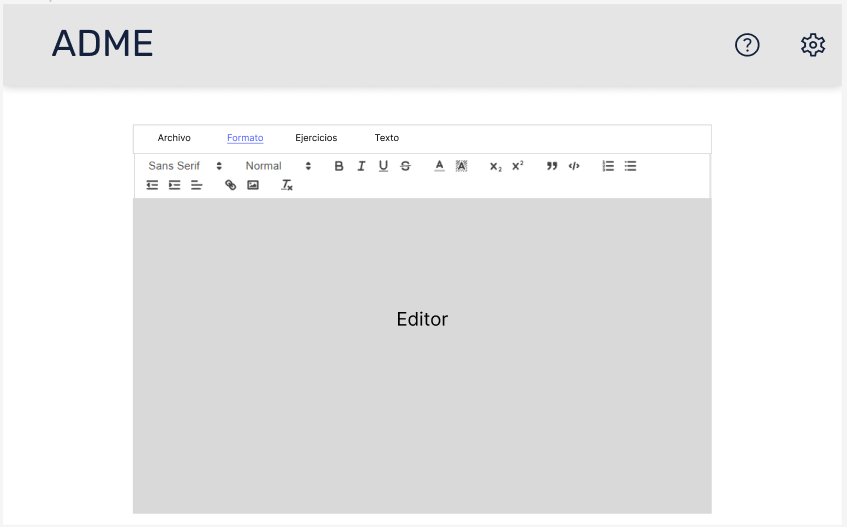
\includegraphics[width=15cm]{Diseño/Pantalla_inicio.png}
  \caption{Diseño final pantalla de inicio.}
  \label{pantallaInicio}
\end{figure}

\begin{figure}[ht!]
  \centering
  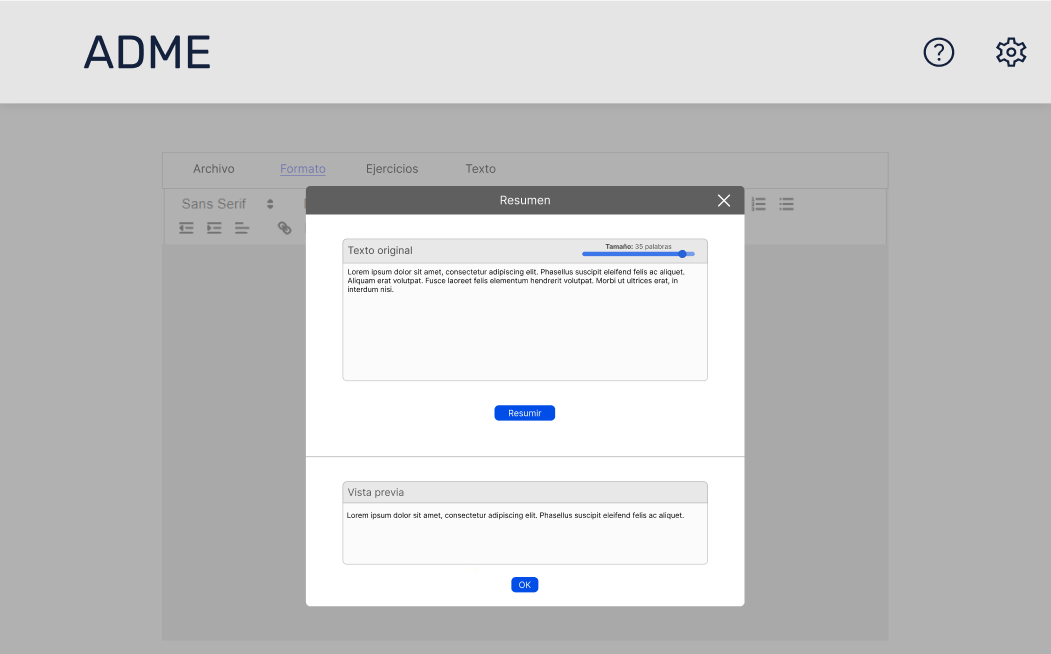
\includegraphics[width=15cm]{Diseño/Resuemn.PNG}
  \caption{Diseño final generar resumen.}
  \label{resuemn}
\end{figure}

\begin{figure}[ht!]
  \centering
  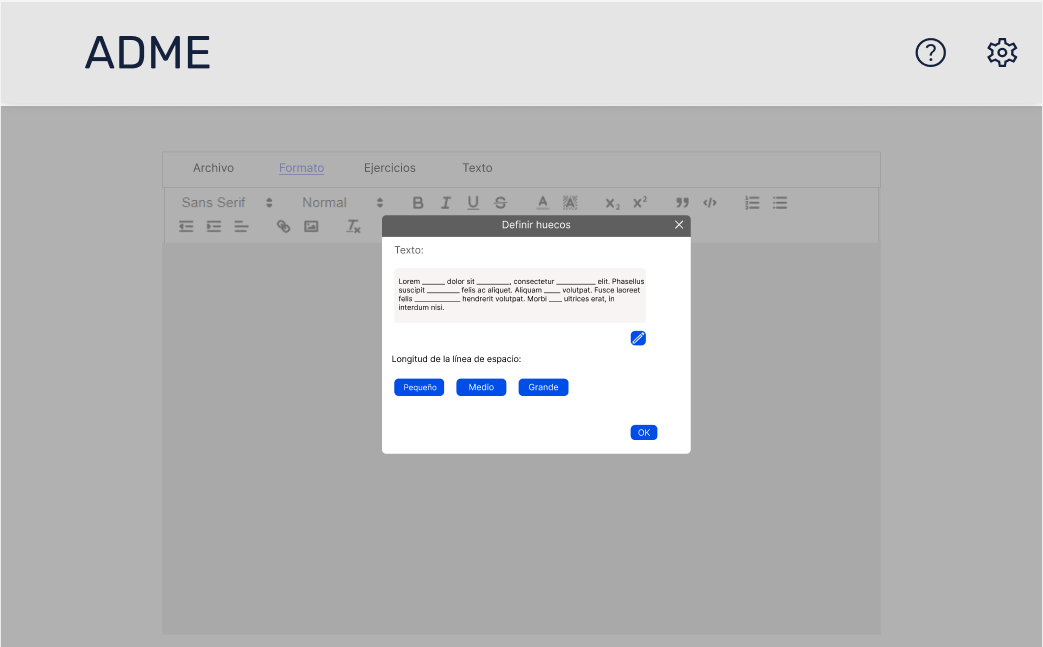
\includegraphics[width=15cm]{Diseño/Definir_huecos.PNG}
  \caption{Diseño final definir huecos.}
  \label{definir_hueco}
\end{figure}

\begin{figure}[ht!]
  \centering
  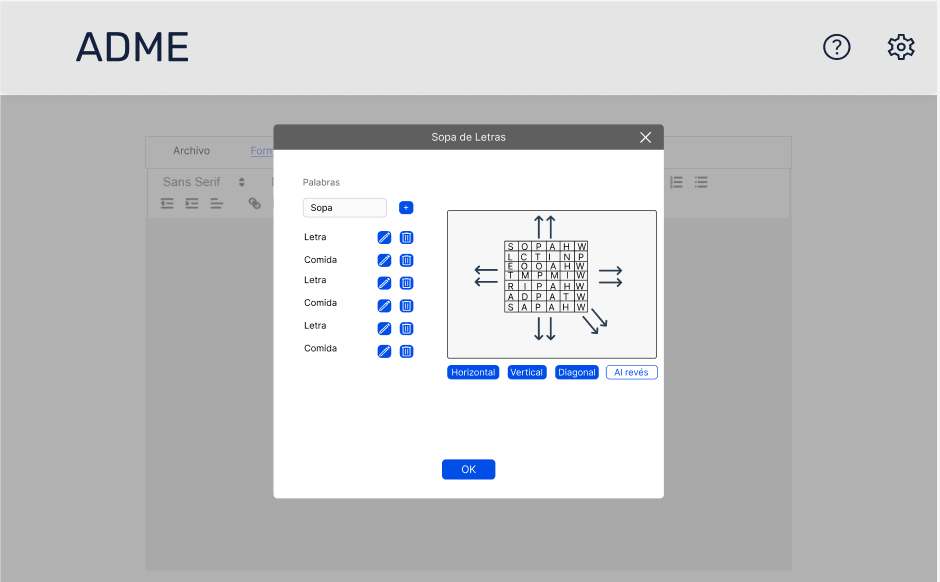
\includegraphics[width=15cm]{Diseño/Sopa_Letras.PNG}
  \caption{Diseño final sopa de letras.}
  \label{sopaLetras}
\end{figure}

\begin{figure}[ht!]
  \centering
  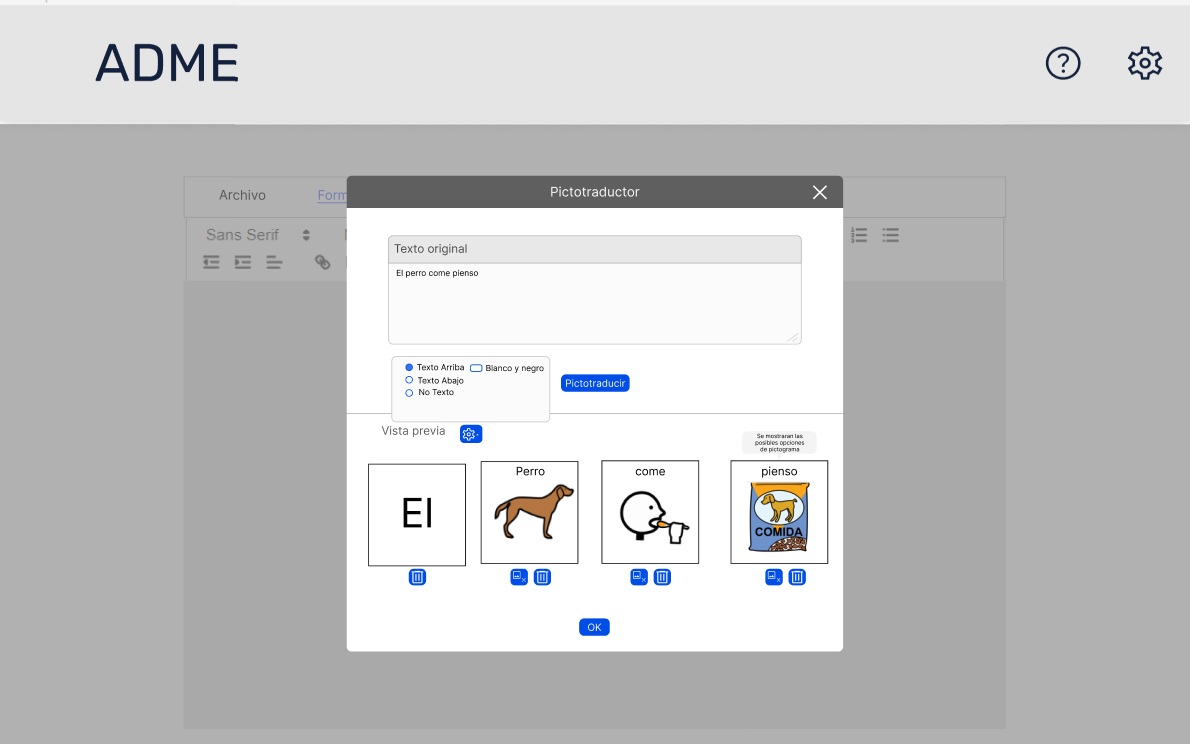
\includegraphics[width=15cm]{Diseño/Pictotraductor.PNG}
  \caption{Diseño final del pictotraductor.}
  \label{pictotraductor}
\end{figure}

\begin{figure}[ht!]
  \centering
  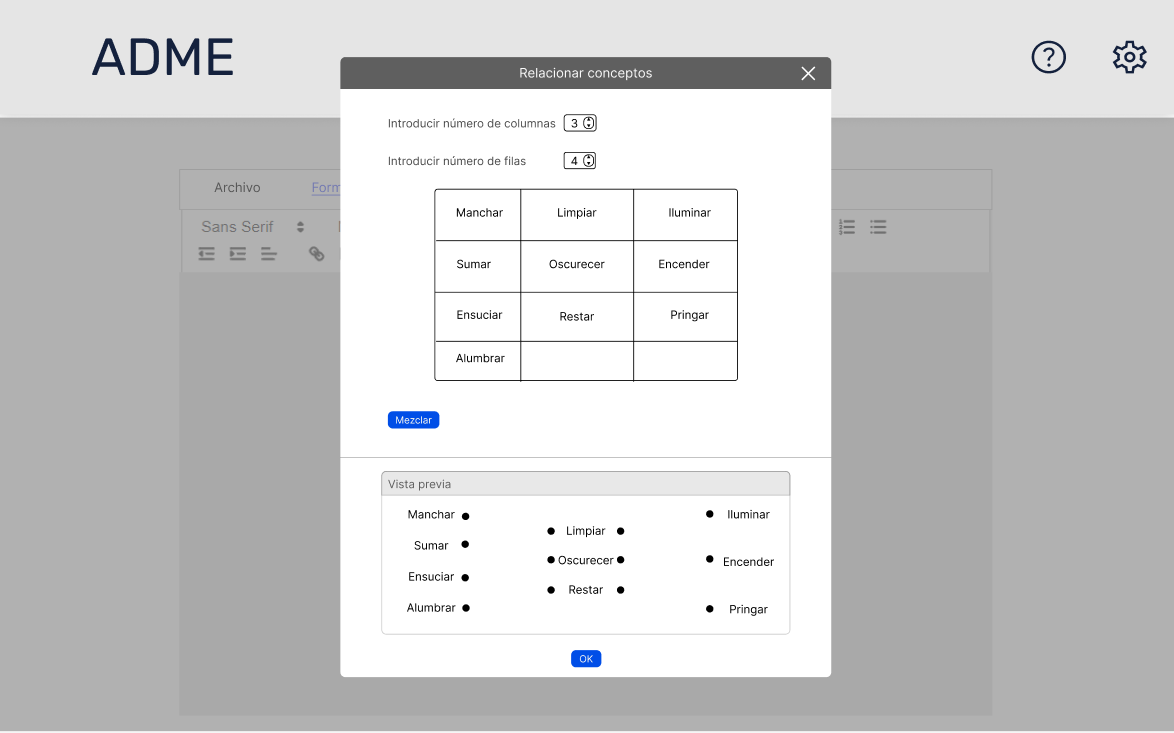
\includegraphics[width=15cm]{Diseño/flechas.png}
  \caption{Diseño final de ejercicios de fechas.}
  \label{flechas}
\end{figure}

\begin{figure}[ht!]
  \centering
  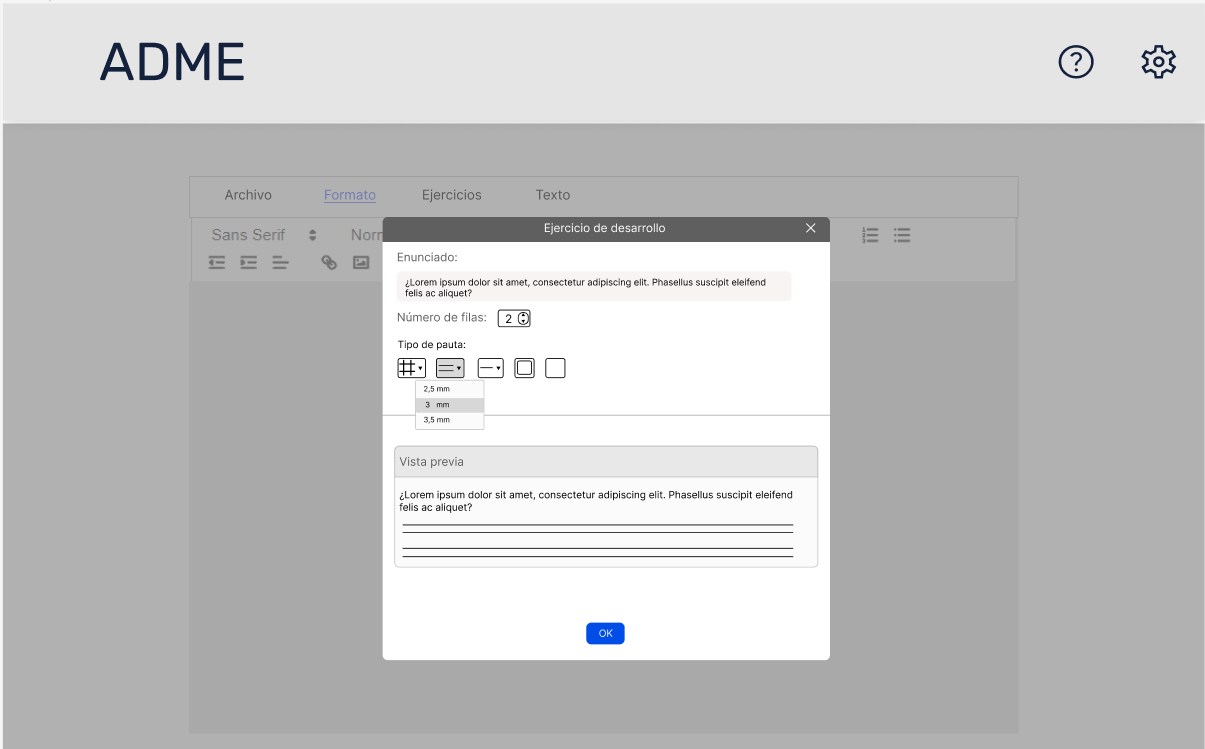
\includegraphics[width=15cm]{Diseño/Desarrollo.PNG}
  \caption{Diseño final de ejercicios de desarrollar.}
  \label{Desarrollo}
\end{figure}

\begin{figure}[ht!]
  \centering
  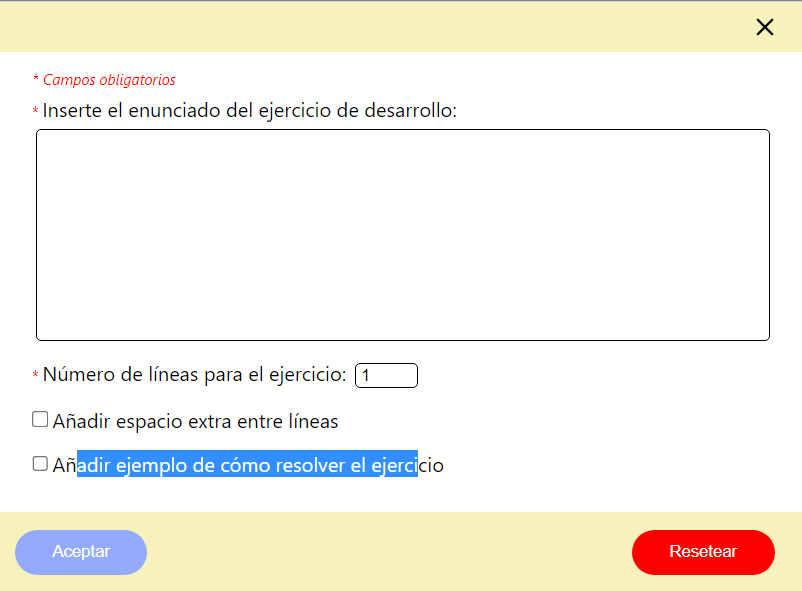
\includegraphics[width=15cm]{Diseño/desarrolloAE1.PNG}
  \caption{Diseño ejercicios de desarrollar AdaptaMaterialEscolar 1.0.}
  \label{desAE1}
\end{figure}

\begin{figure}[ht!]
  \centering
  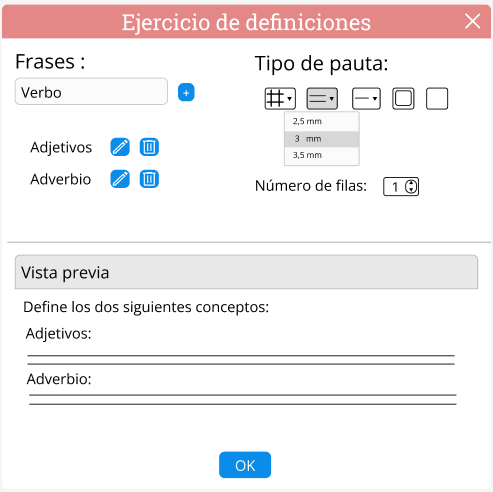
\includegraphics[width=15cm]{Diseño/definiciones.PNG}
  \caption{Diseño final ejercicios de definiciones.}
  \label{defi}
\end{figure}

\begin{figure}[ht!]
  \centering
  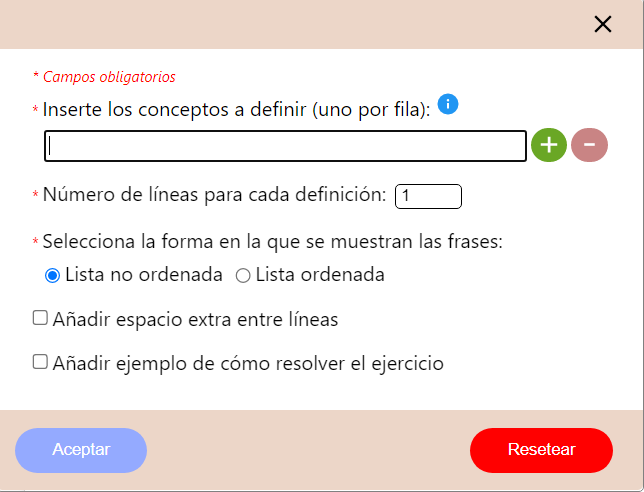
\includegraphics[width=15cm]{Diseño/definicionesAE1.PNG}
  \caption{Diseño ejercicios de definiciones AdaptaMaterialEscolar 1.0.}
  \label{defiAE1}
\end{figure}

\begin{figure}[ht!]
  \centering
  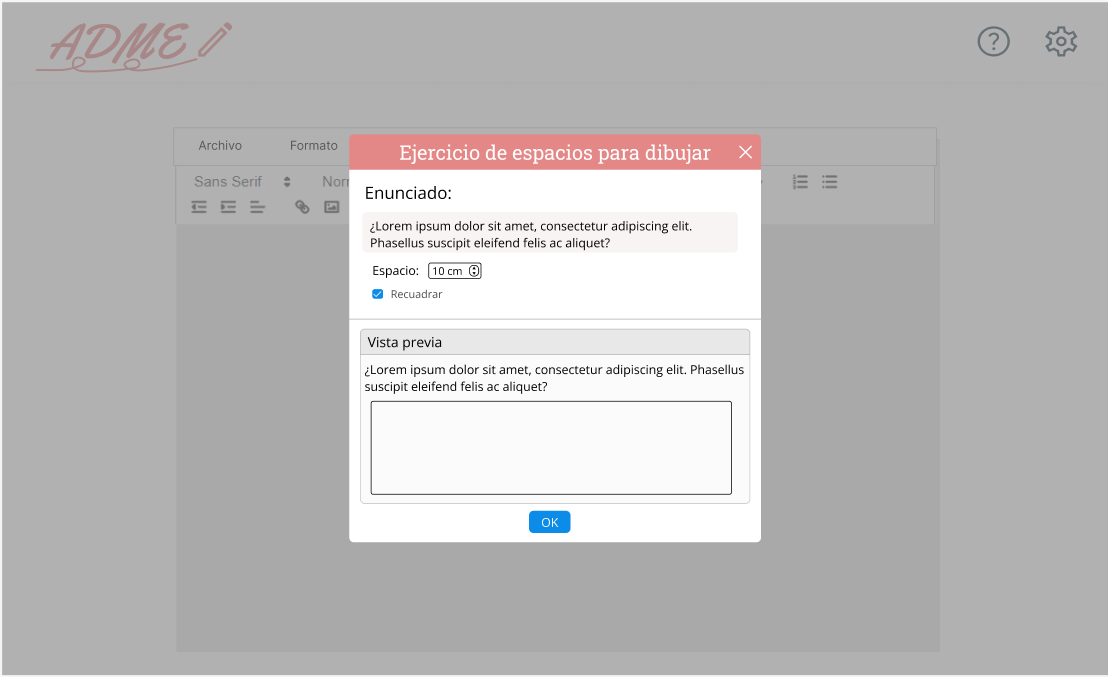
\includegraphics[width=15cm]{Diseño/EspacioDibu.PNG}
  \caption{Diseño final ejercicios espacios para dibujar.}
  \label{espaciosDibu}
\end{figure}

\begin{figure}[ht!]
  \centering
  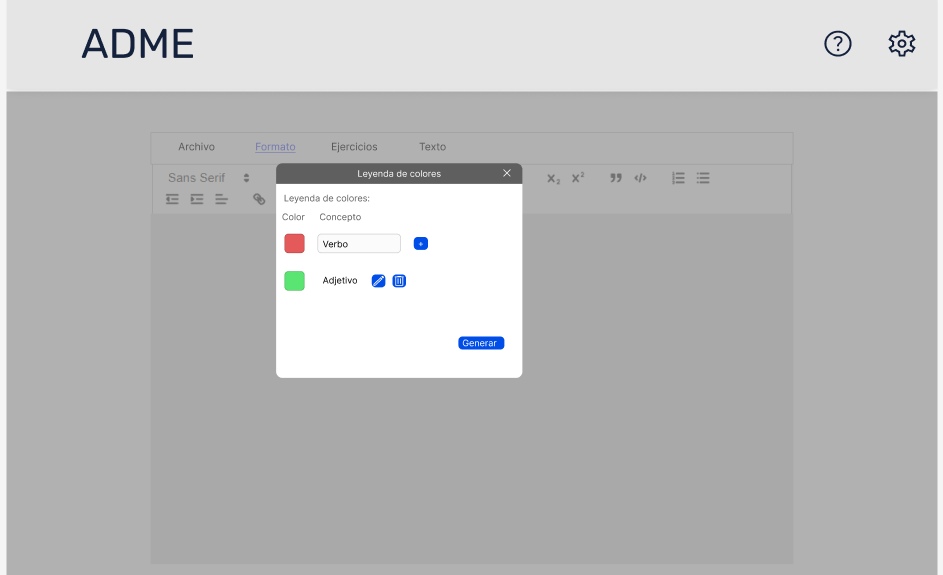
\includegraphics[width=15cm]{Diseño/LeyendaColores.PNG}
  \caption{Diseño final leyenda de colores.}
  \label{espaciosDibu}
\end{figure}


\begin{figure}[ht!]
  \centering
  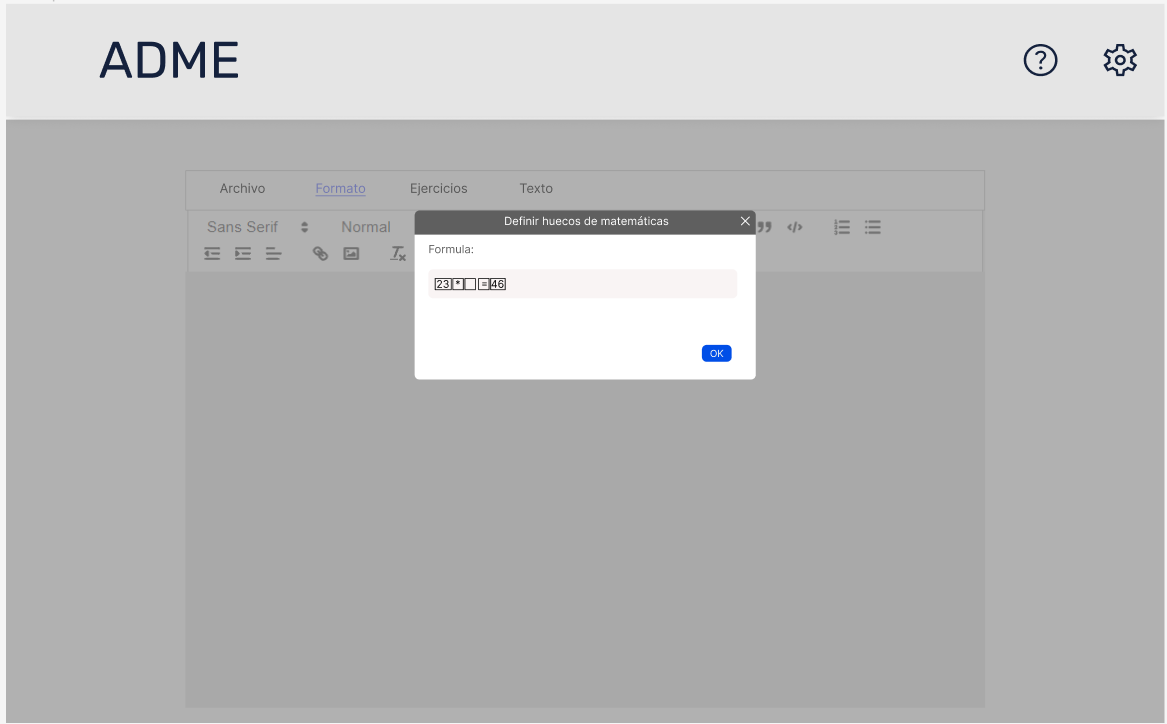
\includegraphics[width=15cm]{Diseño/EjercicioMateHueco.PNG}
  \caption{Diseño final ejercicios de matemáticas con huecos.}
  \label{matesHueco}
\end{figure}

\begin{figure}[ht!]
  \centering
  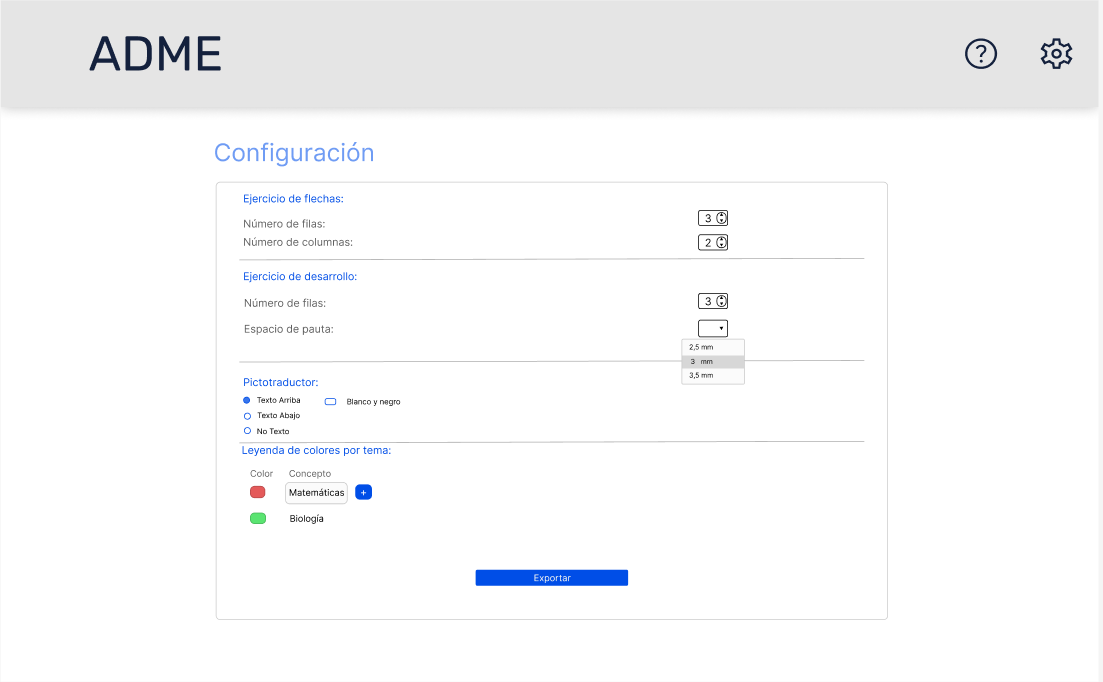
\includegraphics[width=15cm]{Diseño/Configuracion.PNG}
  \caption{Diseño final de la configuración general.}
  \label{configu}
\end{figure}



